\documentclass[10pt]{article}

\linespread{1} 
\usepackage{float}

\usepackage{geometry}
 \geometry{
  papersize={175mm,248mm},
 total={175mm,248mm},
 left=26mm,
 right=13mm,
 bottom=17mm,
 top=13mm,
 }

\usepackage{amsfonts,amssymb,graphicx,color}
\usepackage[font=small,labelfont=bf]{caption}
\usepackage{subcaption}

\usepackage{color, colortbl, framed}
\usepackage[T1]{fontenc}
\usepackage{mathptmx}

\usepackage{amsmath}
%\usepackage{lineno,hyperref}
\usepackage{authblk}
\usepackage{titlesec}

%\usepackage{epstopdf}

\usepackage{hhline}
\usepackage{xcolor,colortbl}
\renewcommand{\figurename}{Fig.}

%  \setcounter{secnumdepth}{0}
\usepackage{titlesec}
\titlespacing{\section}{0pt}{\parskip}{-\parskip}
\titlespacing{\subsection}{0pt}{\parskip}{-\parskip}
 \titleformat*{\section}{\normalfont\fontfamily{ptm}\fontsize{10}{19}\bfseries}
 \titleformat*{\subsection}{\normalfont\fontfamily{ptm}\fontsize{10}{18}\bfseries}


 \usepackage[numbers,sort&compress,square]{natbib}
 \setlength{\bibsep}{0.0pt}


\usepackage{authblk}
\usepackage{varwidth}

\renewcommand*{\Authsep}{, }
\renewcommand*{\Authand}{, }
\renewcommand*{\Authands}{, }
\renewcommand*{\Affilfont}{\normalsize\normalfont}
\renewcommand*{\Authfont}{\normalsize\normalfont\bfseries}
\setlength{\affilsep}{0em}

\renewcommand{\abstractname}{}    % clear the title
\makeatletter
\renewcommand{\maketitle}{\bgroup\setlength{\parindent}{0pt}
\begin{flushleft}
  \textbf{\@title}
\vspace{10pt}

  \@author
\end{flushleft}\egroup
}
\makeatother


\title{\fontsize{16pt}{10pt}\selectfont\flushleft \textbf{Automatic calculation of thresholds for load dependent condition indicators by modelling of probability distribution functions - maintenance of gearboxes used in mining conveying system} }
% \author{}
\author[1]{Jacek Wodecki}
\author[2]{Pawe{\l} Stefaniak}
\author[3]{Anna Michalak}
\author[4]{Agnieszka Wy{\l}oma{\'n}ska}
% \author[1]{Rados{\l}aw Zimroz}

% \affil[1]{Faculty of Geoengineering, Mining and Geology, Wroclaw University of Science and Technology, Na Grobli 15, 50-421 Wroclaw, Poland}
\affil[1,2,3]{KGHM Cuprum Ltd, R{\&}D Centre, Sikorskiego 2-8, 53-659 Wroclaw, Poland}
\affil[4]{Faculty of Pure and Applied Mathematics, Hugo Steinhaus Center, Wroclaw University of Science and Technology, 50-370 Wroclaw, Poland
\protect\\
\textbf{E-mail:} $^{1}${jwodecki@cuprum.wroc.pl}, $^{2}${pkstefaniak@cuprum.wroc.pl},\protect\\$^{3}${amichalak@cuprum.wroc.pl}\\ $^{4}${agnieszka.wylomanska@pwr.edu.pl}} 
 
\date{} 

\begin{document}

\maketitle

\textbf{Abstract.} Limit values for gearbox vibration-based condition indicators are key to determine in order to be able to estimate moment when object is in a need of maintenance. Further decision making process usually might utilize simple \textit{if-then-else} rule using established threshold values. If diagnostic data takes the values from the Gaussian distribution, finding the decision boundaries is not difficult. Simplistically, that comes down to standard pattern recognition technique for "good condition" and "bad condition" based on probability density functions (\textit{PDFs}) of diagnostic data. This situation is becoming more and more complicated when distribution is not Gaussian. Such cases require to develop much more advanced analytically solution. In this paper we present the case of belt conveyor's gearbox for which \textit{PDFs} of diagnostic features overlap each other because of strong influence of time varying operating conditions on spectral features. New approach to automatic threshold recognition has been proposed based on modeling diagnostic features with Weibull distribution and using agglomerative clustering to distinguish classes of technical condition, which leads to determination of thresholds separating them.
\newline \newline
\textbf{Keywords:} gearbox, Weibull distribution, condition monitoring, statistical analysis, clustering.

\section{Introduction}

Condition - Based Maintenance (\textit{CBM}) is the subject of growing interest in the industry. Initially, such approach was used only in case of the most critical machines based on simple statistics of vibration signals like \textit{RMS}, \textit{skewness} or \textit{kurtosis}. Over time, monitoring systems were developed with special dedication to specific groups of machines both in online as well as periodic acquisition form and were applied to more and more objects of machinery park. Today, \textit{CBM} comes down to data fusion -- dozens of variables are acquired simultaneously from each object in real time. For maintenance and management purposes the key issue is to propose such set of indicators calculated from measured time series which will enable complete and objective evaluation of objects in technical, economic and organization aspects as well as estimation of their residual life time. On industrial scale, it very often takes the form of so called big data solution \cite{bartkowiak2014dimensionality}. Another challenge is related to established thresholds for these condition indicators what usually requires to use a data-driven approach. In this paper we will present procedure for setting optimal thresholds for diagnostic features proposed to compound diagnosis of gearboxes used in mining conveying system. In the literature this problem is well-known. \cite{marhadi2013simple} discussed that there exist some kind of limit values which can be identified based on statistics. In simple terms, distribution of vibration data takes the values from the \textit{Gaussian} distribution. In such classical case decision making regarding the technical condition of object is simple. That requires only usage of standard pattern recognition technique for "good condition" and "bad condition" based on probability density functions of features. \cite{zimroz2014diagnostics} pointed out the fact that in case of time varying operating conditions, alarm threshold for spectral features should be determined using load susceptibility characteristics (\textit{LSCh}) of monitored object which can be estimated by linear regression model, while load of conveyor has been deeper analyzed in \cite{krol2017testing}. Classical approach is not sufficient because the \textit{PDFs} of diagnostic features overlap each other. \cite{jablonski2013modeling, stefaniak2016diagnostic,stefaniak2015procedures} propose methodology for recognition of decision boundaries based on \textit{LSCh} for large scale monitoring system including spatially distributed machinery park. They explained that measured features have significantly different probability function from Gaussian. The necessity of data modelling to determine alarm threshold has been shown by \cite{cempel1990limit}, where he considered threshold setting using \textit{Chebyshev's inequality}, \textit{Weibull} and \textit{Pareto} distributions. On the other hand, arguments in favor of other distributions, especially heavy-tailed ones, has been made in \cite{wylomanska2016application}.

Majority of aforementioned cases require to choose the most appropriate distribution of diagnostic data before limit value can be estimated. In \cite{jablonski2013modeling} it has been shown a goodness-of-fit test which allows to chose the most adequate one. 
In this paper authors extend the previous work regarding technical condition assessment, however until now condition classes have been defined manually after visual inspection of empirical tail distribution (see \cite{stefaniak2016diagnostic,stefaniak2015procedures}). Presented methodology allows to define them automatically in a data-driven manner.

The paper is organized as follows: a short technical and operating aspects of machinery park will be described; then remarks and assumptions about automatic threshold finding will be formulated and the methodology will be proposed; industrial data and procedure to calculation of diagnostic features will be shown; finally application of the method will be provided and results will be discussed.

\subsection{Mining conveying system and proposed monitoring system}
\begin{figure}[!ht]
  \centering
  \begin{subfigure}[b]{0.57\textwidth}
      \centering
     % \captionsetup{skip=0.01pt}
      \includegraphics[width=\textwidth]{wykresy/ga}
      \caption{Diagram of the vibration data acquisition module with an exemplary arrangement of the measurement points}
      \label{fig:Raw_map}
  \end{subfigure}
  %\hfill
  \begin{subfigure}[b]{0.4\textwidth}
      \centering
    %  \captionsetup{skip=0.01pt}
		\includegraphics[width=\textwidth]{wykresy/gb}
        \caption{Real object in underground mine during measurement}
    \label{fig:Selectedinterpmap}
  \end{subfigure}
  \vspace{-5pt}
  \caption{Object under investigation}
  \label{fig:raw_interp_map}
\end{figure}

Investigated case study is belt conveyor transportation system using in one of the Polish underground mines of copper ore. Whole conveying system consists of over 80 technical objects combined in transportation network which has the total routes length of 50 km. Their reliability is critical - serious failure of single conveyor might stop operation of whole conveyor division in mine as well as cause of long-term breakdowns of mining processes in mining area or processing plant. One of the most critical conveyor components are gearboxes. As part of proactive tasks, a large-scale monitoring system for drive units has been developed. Because of number of technical objects and their spatial distribution, application of advanced approaches operating online is very difficult and too expensive. For this reason, portable solution has been proposed. Measurements have been performed by using three accelerometers placed orthogonally on the housings of gearboxes. Duration of measurements was equal to 60 seconds. Its sensors layer includes 3 accelometers assembled for gearbox body and tachometric probe directed toward gearbox input shaft (see Fig. \ref{fig:Raw_map},b). Quick measurement delivers 3 vibration signals and tachometric signal.



\section{Methodology}

In this chapter methodology is described. After acquiring raw vibration signal, it is transformed into diagnostic feature carrying information about bearings' technical condition as described in section \ref{df}. After that, for each measurement its empirical tail is calculated, and the outliers are rejected based on fitting Weibull distribution to the tails (see section \ref{weib}). In the next step central points of tails are determined and clustered along with shaft rotational speed, that allows to determine classes of technical condition (see section \ref{clust}).
Key aspects of the method are described in the following sections. 

\subsection{Diagnostic feature}
\label{df}

Processing of raw vibration signals comes down to diagnostic features extraction from vibration signals and calculation of rotational speed of gearbox input shaft from tachometric data in order to identify operating condition. Developed feature extraction procedure is based on segmentation of raw signal dividing it into 60 equal segments without overlapping. Next, each single 1 sec. segment of the signal is transformed into frequency domain iteratively and all components are summed in given spectrum frequency bands (for shafts: 10-100 Hz, for gears: 100-3500 Hz, for bearings: 3500-10000 Hz). Finally, 60 sec. time series of three diagnostic features are extracted: \emph{DF1} (shafts condition), \emph{DF2} (gears condition) and \emph{DF3} (bearings condition). In this work attention is focused on the analysis of \textit{DF3} feature.

\subsection{Fitting Weibull distribution to ECDF tails, MSE rejection}
\label{weib}
First step is to fit translated Weibull distribution to diagnostic features. Density function of translated Weibull distribution is defined as follows:


\begin{equation}
\label{weibull}
    f(x)=\frac{\tau}{\beta} \left( \frac{x-m}{\beta} \right)^{\tau -1} e^{-\left ( \frac{x-m}{\beta} \right)^{\tau}},\qquad x\geqslant m,
\end{equation}
where $m \in \mathbb{R}$ is a shift parameter, $\beta>0$ is scale parameter and $\tau>0$ is a shape parameter \cite{coles2001introduction}. In the field of condition monitoring, Weibull distribution found interesting applications e.g. in time-to-failure modelling \cite{sikorska2011prognostic,wang2002model,zhou2013transformer}. The idea of estimation the parameters is described in \cite{stefaniak2016diagnostic}. Next, we analyze the quality of fit by calculate mean square error (MSE) between empirical tail of diagnostic features and theoretical one given by: 
\begin{equation}
\label{tail}
    T(x)=P(\textbf{X}>x)= e^{-\left ( \frac{x-m}{\beta} \right)^{\tau}},\qquad x\geqslant m.
\end{equation}
We choose such diagnostic features for which the calculated MSEs exceed the given threshold and we reject it.


\subsection{Central point and clustering}
\label{clust}
Core idea of automatic distinction of wear levels based on distribution tails incorporates tails clustering based on their distribution along the diagnostic feature value. Since tails take values between 0 and 1, it is reasonable to estimate tail location as its central point, being the argument of tail value equal to 0.5 (see Fig. \ref{fig:tails}). 

\begin{figure}[h!]
\centering
\includegraphics[width=0.4\textwidth]{wykresy/agl}
\caption{Flowchart of aglomerative hierarchical algorithm}
\label{fig:agl}
\end{figure}

When locations of tails are determined, they are clustered into three clusters using agglomerative clustering algorithm \cite{kaufman2009finding,rokach2005clustering}. The number of clusters is determined by three expected condition states: healthy, warning and alarm (approaching failure). Agglomerative hierarchical clustering is a bottom-up clustering method where clusters have sub-clusters, which in turn have sub-clusters, etc. The classic example of this is species taxonomy. Gene expression data might also exhibit this hierarchical quality (e.g. neurotransmitter gene families). Agglomerative hierarchical clustering starts with every single object (gene or sample) in a single cluster. Then, in each successive iteration, it agglomerates (merges) the closest pair of clusters by satisfying some similarity criteria, until all of the data is in one cluster (see Fig. \ref{fig:agl}).


An alternative top-down hierarchical clustering method is less commonly used. It works in a similar way to agglomerative clustering but in the opposite direction. This method starts with a single cluster containing all objects, and then successively splits resulting clusters until only clusters of individual objects remain.

\section{Results}

\begin{figure}[h!]
\centering
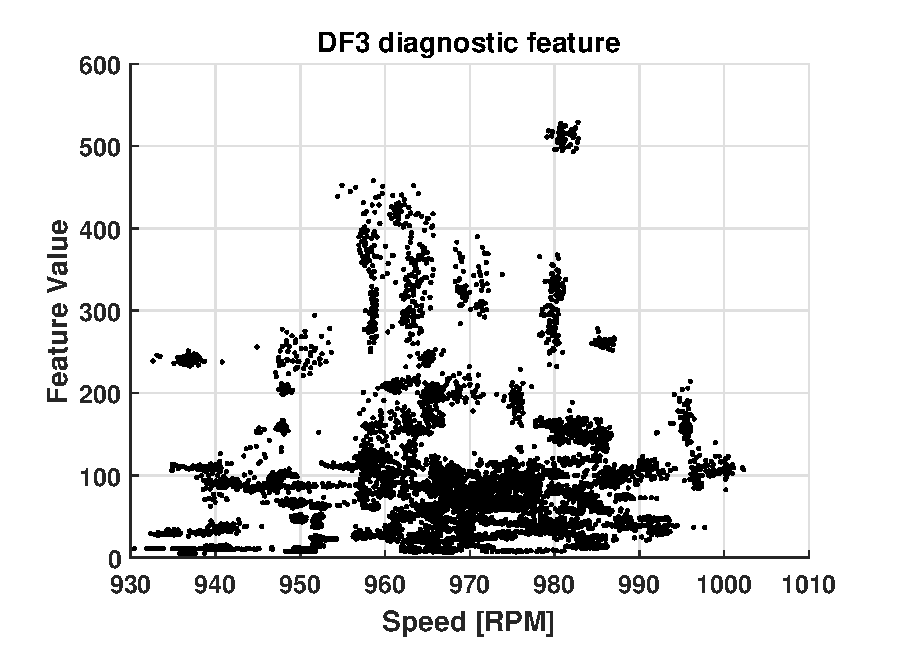
\includegraphics[width=0.7\textwidth]{wykresy/df3}
\caption{Raw diagnostic feature data; dataset consists of 155 measurements, each represented as a point cloud of 60 points corresponding to 60 seconds of a measurement}
\label{fig:df3}
\vspace{-5pt}
\end{figure}


Firstly, diagnostic feature of interest has been obtained from raw vibration signal according to the description in section \ref{df} (see Fig. \ref{fig:df3}).

\begin{figure}[h!]
\centering
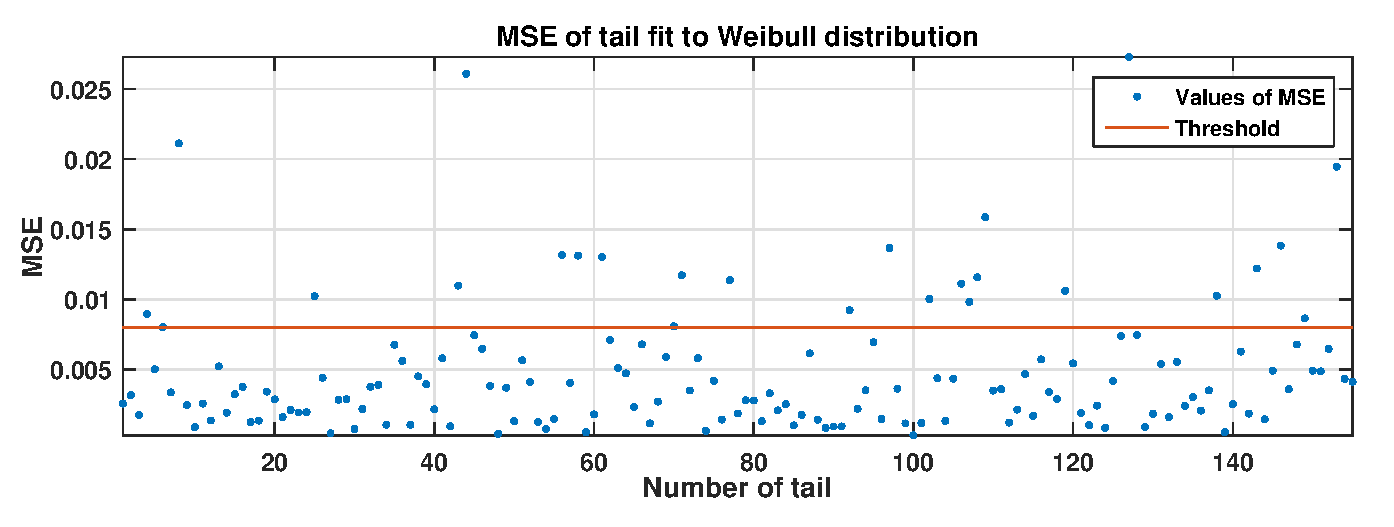
\includegraphics[width=0.8\textwidth]{wykresy/mse}
\vspace{-10pt}
\caption{MSE values for tail fitting}
\label{fig:mse}
\vspace{-5pt}
\end{figure}

In the next step a tail of ECDF was calculated for \textit{DF3} points of each measurement. Weibull distribution was fitted to each tail, and tails with the greatest fit errors have been disregarded (see Fig. \ref{fig:mse}). For remaining tails, middle point value was calculated and complete set of middle points was provided to the clustering algorithm (see Fig. \ref{fig:tails}).



\begin{figure}[h!]
\centering
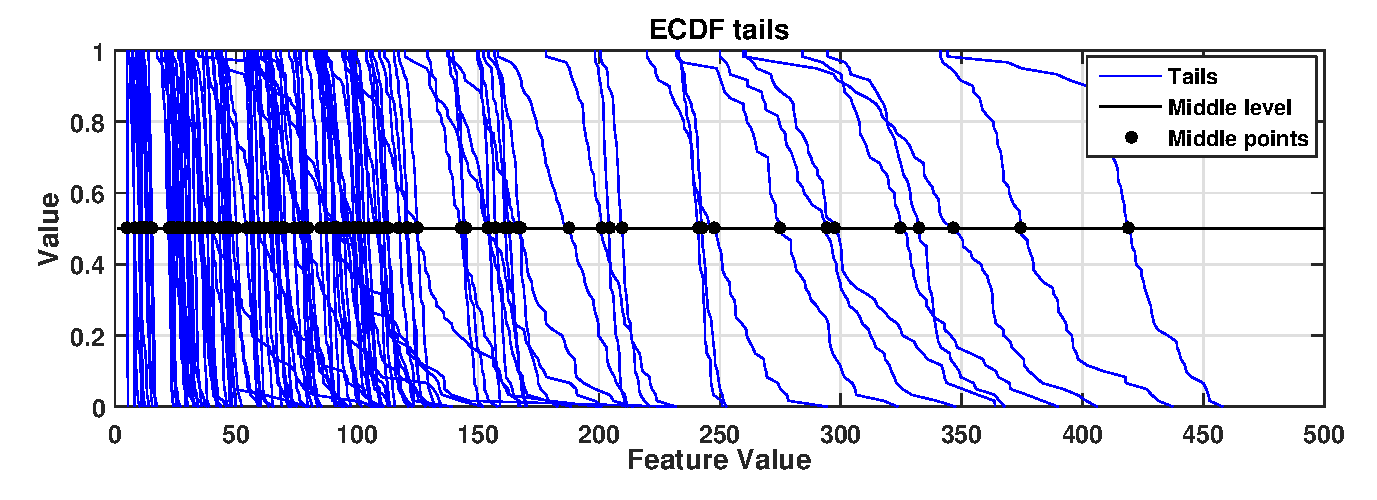
\includegraphics[width=0.8\textwidth]{wykresy/tails}
\vspace{-10pt}
\caption{ECDF tails with marked locations on half-magnitude level}
\label{fig:tails}
\vspace{-5pt}
\end{figure}
% \vspace{-10pt}

As a result, tails have been classified into three clusters indicating different health states (see Fig. \ref{fig:out} right panel). This information was then translated into the two-dimensional plane of \textit{DF3} values vs. RPM, which has been divided into three sectors (see Fig. \ref{fig:out} left panel). Sectors' edges were determined as weighted means between linear fits of two adjacent clusters, where weights were the variance values of \textit{DF3} coordinates of clusters' members. For each pair of adjacent clusters, weights were normalized by their sum.

As a result, technical condition evaluation map has been constructed. It can be used as a condition evaluation basis for future measurements to be obtained, upon which the map can be dynamically updated.

\begin{figure}[h!]
\centering
\includegraphics[width=0.8\textwidth]{wykresy/out.png}
\vspace{-5pt}
\caption{Results of condition regimes classification. Left panel: Measurements as a diagnostic feature in a function of rotational speed. Each dot represents a point cloud of a single measurement and is its centroid. Linear regression functions for each cluster allow to determine the borderlines between adjacent clusters. Right panel: Empirical tails of measurements.}
\label{fig:out}
\end{figure}
\vspace{-10pt}
% \begin{figure}[!ht]
%   \centering
%   \begin{subfigure}[b]{0.5\textwidth}
%       \centering
%      % \captionsetup{skip=0.01pt}
%       \includegraphics[width=\textwidth]{Raw_map2}
%       \caption{Input data in time-time domain}
%       \label{fig:Raw_map}
%   \end{subfigure}
%   %\hfill
%   \begin{subfigure}[b]{0.38\textwidth}
%       \centering
%     %  \captionsetup{skip=0.01pt}
% 		\includegraphics[width=\textwidth]{Selected_interp_map}
%         \caption{Selected interpolated shifts}
%     \label{fig:Selectedinterpmap}
%   \end{subfigure}
%   \caption{Raw temperature data restructured to time-time domain (panel a) and the same map after shift selection and interpolation (panel b)}
%   \label{fig:raw_interp_map}
% \end{figure}

\section{Conclusions}
The paper concerns significant issue of condition monitoring related to making diagnosis based on vibration signal, namely identification of thresholds for diagnostic features. The authors consider gearboxes used in mining conveying system for which strong influence of time varying operating conditions on spectral features cause that well-known methods are ineffective. Proposed approach is based on statistical modeling of diagnostic data set from a single measurement. After disregarding outliers based on goodness of tails fit to Weibull distribution, dataset is clustered to distinguish separate classes of technical condition. Statistical analysis allows to determine boundaries of those classes after the separation. Results perfectly correspond with previously obtained ones that utilized manual classification and thresholding.

\section*{Acknowledgement}
This work is supported by the Framework Programme for Research and Innovation Horizon 2020 under grant agreement n. 636834 (DISIRE - Integrated Process Control based on Distributed In-Situ Sensors into Raw Material and Energy Feedstock) 


\bibliographystyle{JVE_style}
\small\bibliography{mybibfile}


\end{document}